\chapter{Fundamentação Teórica}

Este capítulo reúne a fundamentação teórica necessária, cobrindo conceitos de computação em nuvem, virtualização, nuvens privadas, arquitetura do OpenStack e princípios de elasticidade e provisionamento dinâmico de recursos.

\section{Visão Geral de Computação em Nuvem}

A computação em nuvem (\textit{cloud computing}) é definida pelo \textit{National Institute of Standards and Technology}(NIST), como um modelo que permite acesso a um conjunto compartilhado de recursos computacionais configuráveis, como redes, servidores, armazenamento, aplicações e serviços,  sob demanda e via rede. Esses recursos podem ser rapidamente provisionados e liberados com mínimo esforço de gerenciamento ou interação com o provedor de serviços \cite{mell2011}. Essa definição enfatiza características essenciais da computação em nuvem, dentre as quais destacam-se: 
\textbf{Autoatendimento sob demanda (\textit{On-demand self-service}):} o usuário pode provisionar recursos computacionais, como tempo de servidor e armazenamento em rede, conforme a necessidade, automaticamente e sem necessidade de interação humana com cada provedor de serviço.
\textbf{Acesso amplo à rede (\textit{Broad network access}):} Os serviços da nuvem podem ser acessados pela grande maioria de aparelhos que possuem acesso à internet, com interfaces padronizadas que facilitam a experiência dos usuários que já estão acostumados com algum serviço na nuvem.
 
\textbf{Agrupamento de recursos (\textit{Resource pooling}):} Os recursos computacionais, como processamento, memória, armazenamento e largura de banda de rede, são agrupados pelo provedor para atender múltiplos inquilinos usando um modelo de multilocação (\textit{multi-tenant}), com diferentes recursos sendo distribuídos dinamicamente e redistribuídos conforme a demanda do inquilino.
\textbf{Elasticidade rápida (\textit{Rapid elasticity}):} Os recursos podem ser provisionados e liberados elasticamente, em alguns casos automaticamente, para escalar rapidamente conforme a demanda. Para o usuário, as capacidades disponíveis para provisionamento parecem ser ilimitadas, a depender da quantidade de hardware que o provedor possui,  e podem ser utilizadas em qualquer quantidade, a qualquer momento. 
\textbf{Serviço mensurado (\textit{Measured service}):} Sistemas de nuvem controlam e otimizam automaticamente o uso de recursos utilizando recursos de medição. Devido a isso, o uso dos recursos pode ser monitorado, controlado e reportado, proporcionando transparência tanto para o provedor quanto para o consumidor do serviço utilizado. 

Além dessas características essenciais, os serviços oferecidos por provedores de nuvem são classificados em modelos de serviço:

\textbf{Software como Serviço (\textit{SaaS})}: é um modelo de distribuição de software onde o software é hospedado na nuvem e disponibilizado aos usuários através da internet. Essa infraestrutura de nuvem é formada por uma camada física, composta por servidores, armazenamento e componentes de rede, e uma camada de abstração, que seria um software implantado sobre essa infraestrutura física \cite{mell2011}. 

\textbf{Plataforma como Serviço (\textit{PaaS})}: é um modelo que fornece ao consumidor a possibilidade de implantar, sobre a infraestrutura de nuvem, aplicações criadas ou adquiridas usando linguagens de programação, bibliotecas, serviços e ferramentas compatíveis com o ambiente oferecido pelo provedor. O consumidor não gerencia nem controla a infraestrutura subjacente da nuvem, como redes, servidores, sistemas operacionais ou armazenamento, mas possui controle sobre as aplicações implantadas e, possivelmente, sobre as configurações do ambiente onde essas aplicações serão hospedadas \cite{mell2011}.

\textbf{Infraestrutura como Serviço (\textit{IaaS})}: é um modelo que fornece ao consumidor a capacidade de provisionar recursos computacionais, como processamento, armazenamento, redes e outros, permitindo que ele implante e execute softwares, incluindo sistemas operacionais e aplicações. O consumidor também não gerencia nem controla a infraestrutura física da nuvem, mas tem controle sobre os sistemas operacionais, o armazenamento, as aplicações implantadas e, em alguns casos, controle limitado de componentes específicos de rede, como firewalls do host \cite{mell2011}.

\begin{figure}[htb]
    \centering
    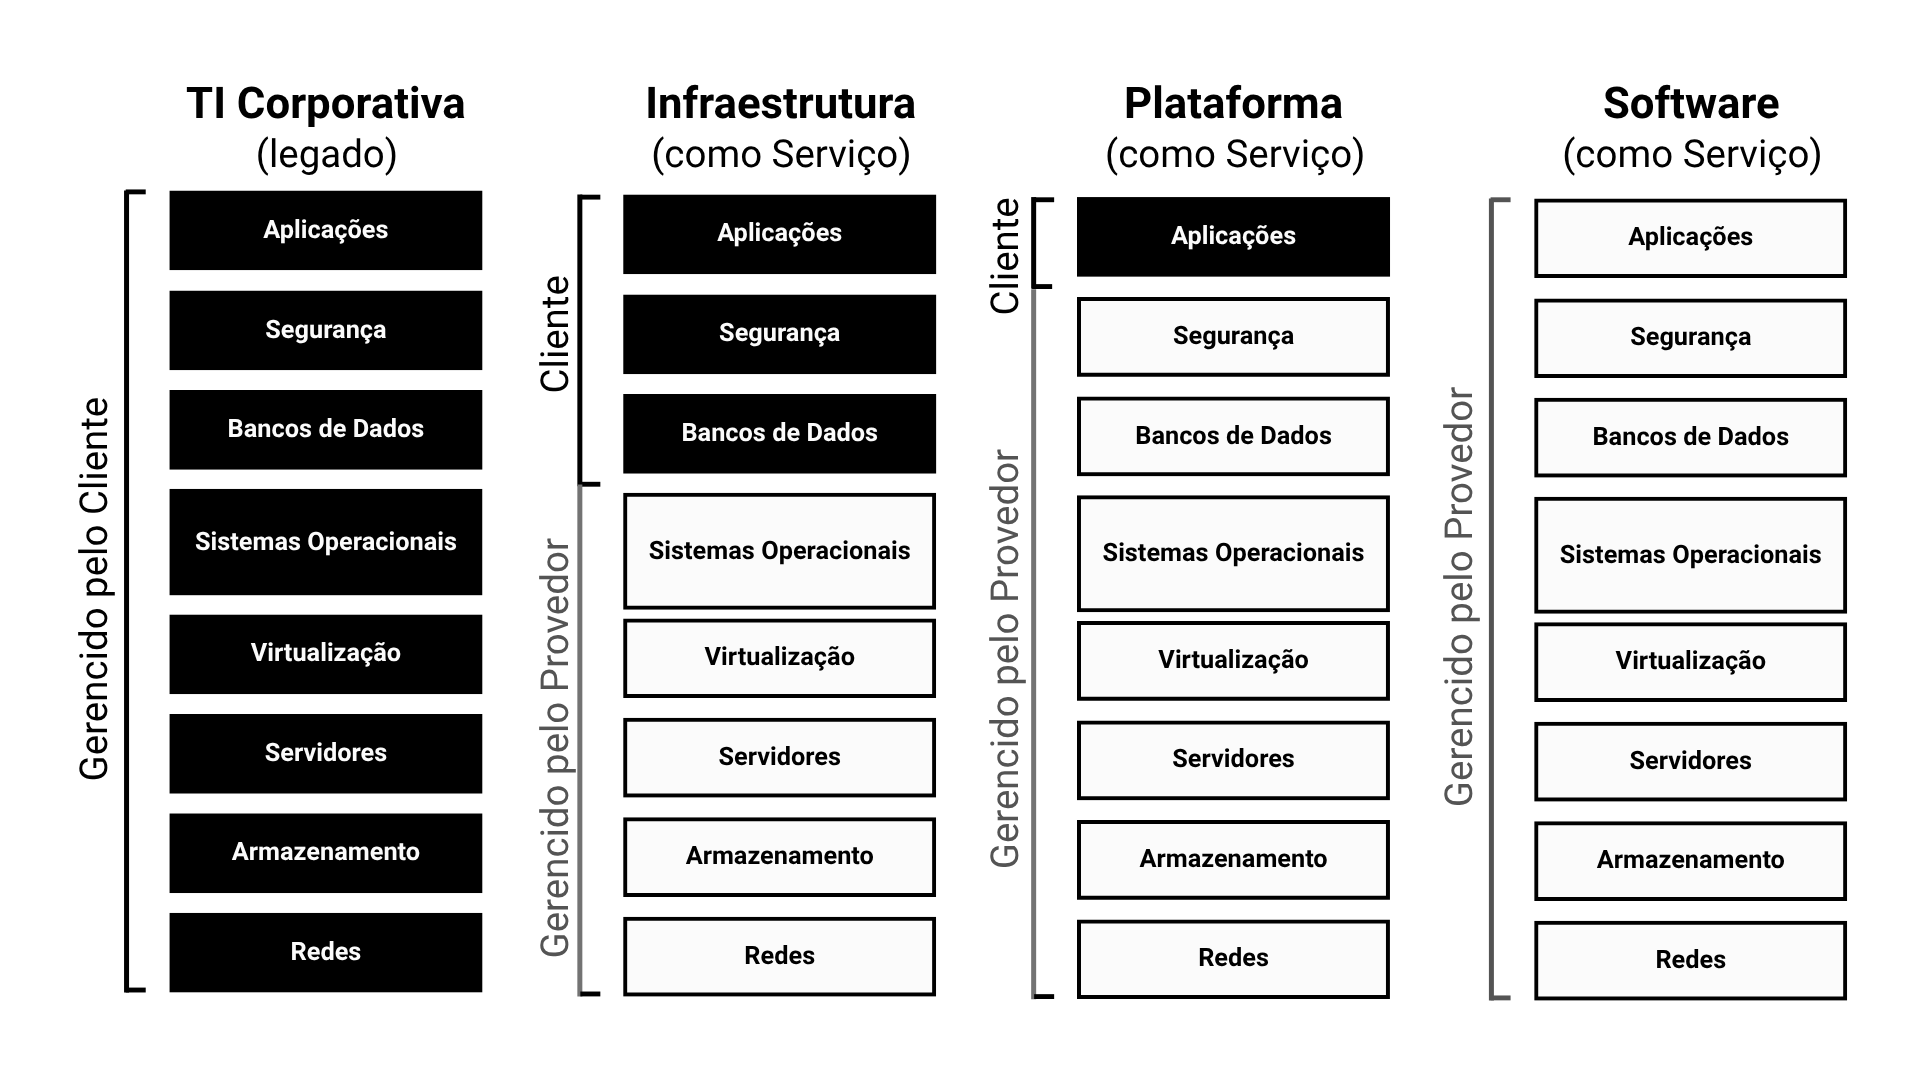
\includegraphics[width=0.8\textwidth]{figuras/Figura 1 - Comparação entre os modelos de serviço.png}
    \caption{Comparação entre os modelos de serviço \textit{IaaS}, \textit{PaaS} e \textit{SaaS}}
    \label{fig:comparacao-modelos-servico}
\end{figure}

Para facilitar o entendimento desses serviços, a Figura \ref{fig:comparacao-modelos-servico} compara os modelos entre si e quais partes da nuvem o usuário tem controle em cada um. Os quadrados verdes representam responsabilidades do usuário, enquanto os azuis são responsabilidades do provedor. Em sistemas de \textit{SaaS}, o usuário não tem responsabilidade nenhuma, mas, em compensação, não gerencia nem controla a infraestrutura da nuvem. Grande parte dos serviços oferecidos a usuários da internet utilizam esse modelo. Dentre eles, pode-se listar as redes sociais, como o \textit{Instagram}, \textit{TikTok} e \textit{Whatsapp}, e serviços de transmissão contínua de conteúdo multimídia (\textit{streaming}), como o \textit{Youtube}, \textit{Netflix} e \textit{Spotify}.  No \textit{PaaS}, o usuário tem controle sobre a aplicação, incluindo códigos e bancos de dados. Nesse modelo encontram-se os serviços de desenvolvimento e hospedagem de software, como \textit{AWS Elastic Beanstalk}, \textit{Google App Engine} e \textit{Heroku}. Já no \textit{IaaS}, o usuário pode solicitar uma quantidade de recursos e tem controle sobre o sistema operacional. Nesse modelo estão as máquinas virtuais e serviços de armazenamento, como  \textit{Amazon Web Services (AWS) EC2 e S3},  \textit{Microsoft Azure Virtual Machines} e  \textit{Google Compute Engine}.

\section{Modelos de Implantação} 
A implantação de sistemas de computação em nuvem pode ser realizada por meio de diferentes modelos. Cada modelo possui características peculiares que determinam sua adequação a contextos específicos. Os modelos mais conhecidos são a nuvem pública, privada, comunitária e híbrida, os quais se diferenciam pelo nível de controle, segurança, escalabilidade e custo de implantação \cite{mell2011}.

As nuvens públicas são gerenciadas por provedores terceirizados que disponibilizam recursos computacionais por meio da internet \cite{carroll2011}. Esses provedores costumam oferecer capacidades elevadas de escalabilidade e custos iniciais mais acessíveis, o que os torna atrativos para diferentes perfis de organizações \cite{amajuoyi2024}. Além disso, esse modelo de nuvem pode ser particularmente vantajoso para instituições que não contam com equipes internas especializadas no assunto ou que optam por não direcionar recursos à aquisição e manutenção de infraestrutura física própria. Em função desses benefícios, a adoção da nuvem pública tem apresentado um crescimento contínuo nos últimos anos \cite{amajuoyi2024}. Entretanto, as nuvens privadas podem apresentar desafios relevantes em termos de segurança e controle sobre a infraestrutura física. A nuvem pública é aberta a todos e sem garantia de alto nível de segurança, podendo trazer riscos à confidencialidade dos dados, à proteção de informações estratégicas e à perda ou roubo de dados, sendo uma opção mais adequada para empresas com "baixas preocupações de segurança" \cite{sathya2023}.

Para organizações que desejam um grau elevado de controle, personalização e alto nível de segurança, as nuvens privadas podem se destacar como uma solução adequada \cite{swapna2023}, consistindo em uma infraestrutura dedicada a uma única organização \cite{mell2011}. Isso possibilita o desenvolvimento de um ambiente seguro e adaptado às exigências particulares de instituições que necessitam resguardar pesquisas sigilosas e proteger a propriedade intelectual. 

\section{Virtualização e Hipervisores}

\section{Máquinas Virtuais \& Imagens}

\section{Arquitetura Essencial do OpenStack}

\section{Elasticidade e Provisionamento Dinâmico}

\subsection{Dimensionamento \textit{automático}}

\subsection{Políticas de \textit{Fair-Share} e \textit{Ballooning}}

\section{Imagens Base Compartilhadas}

\section{Trabalhos Relacionados}

\section{Síntese dos Conceitos}
